%%%%%%%%%%%%%%%%%%%%%%%%%%%%%%%%%%%%%%%%%%%%%%%%%%%%%%%%%%%%%%%%%%%%%%%%
%                                                                      %
%     File: Thesis_Implementation.tex                                  %
%     Tex Master: Thesis.tex                                           %

%%%%%%%%%%%%%%%%%%%%%%%%%%%%%%%%%%%%%%%%%%%%%%%%%%%%%%%%%%%%%%%%%%%%%%%%

\chapter{Interoperability}
\label{chapter:interoperability}
\section{Overview}
\label{section:overview}
Resources need to interact to accomplish collaboration, either designed or emergent. This necessarily entails some form of mutual knowledge and understanding, but this creates dependencies on other resources that may hamper resource evolution and that's why Interoperability, a necessary condition to achieve integration between different systems. Another important factor for integration between systems is decoupling which says that resources need to be independent to evolve freely and dynamically. Unfortunately, independent resources do not understand each other and are not able to interact. Therefore, the fundamental problem of resource integration is to provide the maximum decoupling possible while ensuring the minimum interoperability requirements.

%%%%%%%%%%%%%%%%%%%%%%%%%%%%%%%%%%%%%%%%%%%%%%%%%%%%%%%%%%%%%%%%%%%%%%%%
\section{Interoperability in SOA and REST}
\label{section:InteroperabilitySOAREST}

Currently, enterprise integration is based on SOA with Web Services and REST with HTTP; the two most used architectural styles for distributed interoperability. These styles use symmetric arrangement in which a sender produces a message according to some schema and the receiver uses the same schema to validate and to get the contents of the message. The message is sent over a channel between sender and receiver. In SOA web services, schema is usual in XML Schema and WSDL. In the REST world, schemas are known as media types but perform the same role. The difference is that, instead of being declared in a separate document referenced by messages, they need to be previously known to the interaction resources, either by being standard or by having been previously agreed. In any case, the schema or media type must be the same at both sender and receiver and therefore imposes coupling between the resources for all its possible values, even if only a few are actually used. In either case, data types need to be fully known by both interacting resources.
\begin{figure}[!htb]
  \centering
  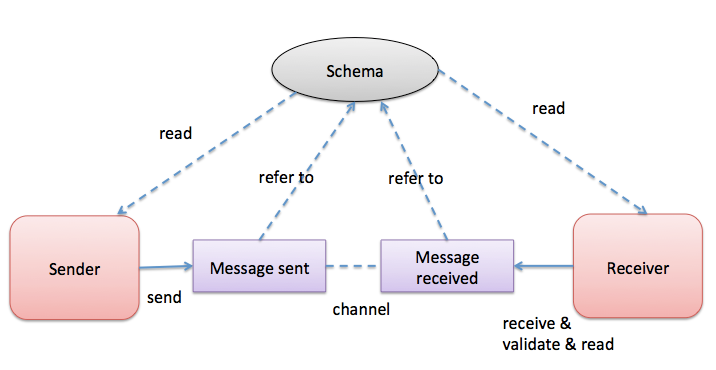
\includegraphics[width=0.9\textwidth]{Figures/schema.png}
  \caption[Interoperability in SOA and REST.]{Interoperability in SOA and REST.}
  \label{fig:interoperability}
\end{figure}

As described above, resources send requests to each other to invoke a given operation with a SOA or REST approach. These requests and their responses usually contain data, which is serialized, sent and reconstructed upon reception of the corresponding message.  The sender and receiver need to interpret those data in a compatible way, which means they need schema. These schemas can be XML Schema and JSON Schema. JSON is a very popular serialization format, as a simpler alternative to XML. JSON Schema is currently just an IETF draft\citep{thesis:arch1}, but is raising interest as a simpler alternative to XML Schema. Both XML and JSON are text based which means inefficient parsing and all characters of a component need to be parsed to reach the next one. Let's explain this with an example, Referring to the example in Chapter \ref{chapter:introduction} that demonstrate interaction between Android mobile phone and .Net weathercast provider. In case of REST approach, An XML or JSON message needed to be created to send server. Lets see how can be created a XML message with Android phone application to send it weathercast provider. The code in Listing ~\ref{lst:javaxml} explains how to create the XML message in Listing ~\ref{lst:xml} with using Java.

\begin{lstlisting}[caption=Example XML message to send weathercast provider, label=lst:xml]

  <?xml version="1.0" encoding="UTF-8" standalone="no" ?>
  <weather>
      <country>Portugal</country>
  		<city>Lisbon</city>
  		<date>30.03.2016</date>
  		<weatherResult></weatherResult>
  </weather>

\end{lstlisting}

\begin{lstlisting}[caption=XML message creation with Java Code, label=lst:javaxml]
  		DocumentBuilderFactory docFactory = DocumentBuilderFactory.newInstance();
  		DocumentBuilder docBuilder = docFactory.newDocumentBuilder();
  		// root elements
  		Document doc = docBuilder.newDocument();
  		Element rootElement = doc.createElement("weather");
  		doc.appendChild(rootElement);
  		// country elements
  		Element country = doc.createElement("country");
  		rootElement.appendChild(country);
  		// city elements
  		Element city = doc.createElement("city");
  		city.appendChild(doc.createTextNode(cityInfo));
  		rootElement.appendChild(city);
  		// date elements
  		Element date = doc.createElement("date");
  		date.appendChild(doc.createTextNode(new Date().toString()));
  		rootElement.appendChild(date);
  		// weatherResult elements
  		Element nickname = doc.createElement("weatherResult");
  		nickname.appendChild(doc.createTextNode(""));
  		rootElement.appendChild(nickname);
  		TransformerFactory transformerFactory = TransformerFactory.newInstance();
  		Transformer transformer = transformerFactory.newTransformer();
  		DOMSource source = new DOMSource(doc); // XML Message
\end{lstlisting}

After creation of XML message with Java, this message will be sent with suitable message level protocol (e.g., HTTP) and will be received by the provider. Weathercast provider will deserialize the message using parsers using schema or pre-agreed standard to understand query message. The code in Listing ~\ref{lst:Cshapxml} explains how to parse an XML message in .Net.

\begin{lstlisting}[caption=XML message parsing with .Net Code, label=lst:Cshapxml]
  string Country;
  string City;
  string date;
  // Create an XmlReader
  using (XmlReader reader = XmlReader.Create(new StringReader(xmlString)))
  {
    reader.ReadToFollowing("weather");
    reader.ReadToFollowing("country");
    Country = reader.ReadElementContentAsString();
    reader.ReadToFollowing("city");
    City = reader.ReadElementContentAsString();
    reader.ReadToFollowing("date");
    date = reader.ReadElementContentAsString();
  }

\end{lstlisting}

As seen in Listing ~\ref{lst:Cshapxml}, the receiver knows the format of XML message. Otherwise it can not deserialize correctly without knowing structure. XML parsing code reads an XML document and uses DOM or SAX APIs\citep{thesis:arch20} to provide programmatic access to its content and structure. After parsing XML message, .Net weathercast provider builds response data as XML message and then send to your mobile phone. Your mobile phone need to parse that XML response message using DOM or SAX API again to display the result on your phone screen. Here in this example it is assumed that both your mobile and weathercast provider know the same schema. Example schema for your mobile phone application and weathercast provider can be as in Listing ~\ref{lst:xmlschema}  and they both first validate message with a validator for example  SAX API validator\citep{thesis:arch10} as seen in Listing ~\ref{lst:javaschemacheck}, otherwise the componenent can not parse XML correctly and can not communicate each other.

\begin{lstlisting}[caption=Example schema for Weather XML file, label=lst:xmlschema]
<xs:schema attributeFormDefault="unqualified" elementFormDefault="qualified" xmlns:xs="http://www.w3.org/2001/XMLSchema">
  <xs:element name="weather">
    <xs:complexType>
      <xs:sequence>
        <xs:element type="xs:string" name="country"/>
        <xs:element type="xs:string" name="city"/>
        <xs:element type="xs:string" name="date"/>
        <xs:element type="xs:string" name="weatherResult"/>
      </xs:sequence>
    </xs:complexType>
  </xs:element>
</xs:schema>
\end{lstlisting}


\begin{lstlisting}[caption=Example XML message to send weathercast provider, label=lst:javaschemacheck]

		SAXParserFactory factory = SAXParserFactory.newInstance();
        factory.setValidating(false);
        factory.setNamespaceAware(true);
        SchemaFactory schemaFactory
                = SchemaFactory.newInstance("http://www.w3.org/2001/XMLSchema");
        factory.setSchema(schemaFactory.newSchema(
                new Source[]{new StreamSource("weather.xsd")}));
        SAXParser parser = factory.newSAXParser();

        XMLReader reader = parser.getXMLReader();
       // reader.setErrorHandler(new SimpleErrorHandler());
        reader.parse(new InputSource("weather.xml"));

\end{lstlisting}

The same example can be implemented with SOA approach. SOA leads to an architectural style that is an evolution of the RPC (Remote Procedure Call) style, by declaring and invoking operations in a standard and language independent way. Service description (WSDL document) must be obtained first by your mobile phone and weathercast provider, so that a contract can be established between that resource (the provider) and the resource that uses it (the consumer). A concrete schema, with the names used, must be specified and be compatible on both sides, otherwise a representation returned by a resource, for example, will not be able to be analyzed and understood.

Webservice will be implemented by .NET for weather cast provider such as in Listing ~\ref{lst:Cshapwebservice} and also following WSDL document will be created automatically for that web service by .NET as seen in Listing ~\ref{lst:wsdldocument}.

\begin{lstlisting}[caption=SOAP Web Service with .Net, label=lst:Cshapwebservice]

  [WebService(Namespace = "http://tempuri.org/")]
  [WebServiceBinding(ConformsTo = WsiProfiles.BasicProfile1_1)]
  public class WebService : System.Web.Services.WebService {
      public WebService () {
      }
      [WebMethod]
      public Weather GetWeatherCast(Weather weather) {
          weather.weatherResult = WeatherCastProvider.GetWeather(weather.country, weather.city, weather.date);
          return weather;
      }
  }
\end{lstlisting}

So if your mobile application knows that WSDL document in Listing ~\ref{lst:wsdldocument}, it can easily call a method from weathercast provider by RPC (Remote Procedure Call) style to get current weathercast info for requested city as shown in Listing ~\ref{lst:javaSOAP}.

\begin{lstlisting}[caption=WSDL Document for Weathercast Provider, label=lst:wsdldocument]
  <?xml version="1.0" encoding="utf-8"?>
  <wsdl:definitions xmlns:tm="http://microsoft.com/wsdl/mime/textMatching/" xmlns:soapenc="http://schemas.xmlsoap.org/soap/encoding/" xmlns:mime="http://schemas.xmlsoap.org/wsdl/mime/" xmlns:tns="http://tempuri.org/" xmlns:soap="http://schemas.xmlsoap.org/wsdl/soap/" xmlns:s="http://www.w3.org/2001/XMLSchema" xmlns:soap12="http://schemas.xmlsoap.org/wsdl/soap12/" xmlns:http="http://schemas.xmlsoap.org/wsdl/http/" targetNamespace="http://tempuri.org/" xmlns:wsdl="http://schemas.xmlsoap.org/wsdl/">
    <wsdl:types>
      <s:schema elementFormDefault="qualified" targetNamespace="http://tempuri.org/">
        <s:element name="GetWeatherCast">
          <s:complexType>
            <s:sequence>
              <s:element minOccurs="0" maxOccurs="1" name="weather" type="tns:Weather" />
            </s:sequence>
          </s:complexType>
        </s:element>
        <s:complexType name="Weather">
          <s:sequence>
            <s:element minOccurs="0" maxOccurs="1" name="country" type="s:string" />
            <s:element minOccurs="0" maxOccurs="1" name="city" type="s:string" />
            <s:element minOccurs="1" maxOccurs="1" name="date" type="s:dateTime" />
            <s:element minOccurs="0" maxOccurs="1" name="weatherResult" type="s:string" />
          </s:sequence>
        </s:complexType>
        <s:element name="GetWeatherCastResponse">
          <s:complexType>
            <s:sequence>
              <s:element minOccurs="0" maxOccurs="1" name="GetWeatherCastResult" type="tns:Weather" />
            </s:sequence>
          </s:complexType>
        </s:element>
      </s:schema>
    </wsdl:types>
    <wsdl:message name="GetWeatherCastSoapIn">
      <wsdl:part name="parameters" element="tns:GetWeatherCast" />
    </wsdl:message>
    <wsdl:message name="GetWeatherCastSoapOut">
      <wsdl:part name="parameters" element="tns:GetWeatherCastResponse" />
    </wsdl:message>
    <wsdl:portType name="WebServiceSoap">
      <wsdl:operation name="GetWeatherCast">
        <wsdl:input message="tns:GetWeatherCastSoapIn" />
        <wsdl:output message="tns:GetWeatherCastSoapOut" />
      </wsdl:operation>
    </wsdl:portType>
    <wsdl:binding name="WebServiceSoap" type="tns:WebServiceSoap">
      <soap:binding transport="http://schemas.xmlsoap.org/soap/http" />
      <wsdl:operation name="GetWeatherCast">
        <soap:operation soapAction="http://tempuri.org/GetWeatherCast" style="document" />
        <wsdl:input>
          <soap:body use="literal" />
        </wsdl:input>
        <wsdl:output>
          <soap:body use="literal" />
        </wsdl:output>
      </wsdl:operation>
    </wsdl:binding>
    <wsdl:binding name="WebServiceSoap12" type="tns:WebServiceSoap">
      <soap12:binding transport="http://schemas.xmlsoap.org/soap/http" />
      <wsdl:operation name="GetWeatherCast">
        <soap12:operation soapAction="http://tempuri.org/GetWeatherCast" style="document" />
        <wsdl:input>
          <soap12:body use="literal" />
        </wsdl:input>
        <wsdl:output>
          <soap12:body use="literal" />
        </wsdl:output>
      </wsdl:operation>
    </wsdl:binding>
    <wsdl:service name="WebService">
      <wsdl:port name="WebServiceSoap" binding="tns:WebServiceSoap">
        <soap:address location="http://localhost:5270/WebService.asmx" />
      </wsdl:port>
      <wsdl:port name="WebServiceSoap12" binding="tns:WebServiceSoap12">
        <soap12:address location="http://localhost:5270/WebService.asmx" />
      </wsdl:port>
    </wsdl:service>
  </wsdl:definitions>
\end{lstlisting}

Developing client side code for given WSDL is usally automatically generated for you by using programming language. When developping code in clinet side, The following steps need to be completed to generate code for given WSDL file in Java.
\begin{itemize}
  \item Click to “Add new file” as seen in Figure \ref{fig:wsdlstep1}.
  \item Choose file type as “Web Service Client”.
  \item Choose WSDL URL and Copy and paste your WSDL URl adress as seen in Figure \ref{fig:wsdlstep2}.
  \item Click Finish.
\end{itemize}

After these steps you can start to write client side code in Java as shown in Listing ~\ref{lst:javaSOAP}.

\begin{lstlisting}[caption=SOAP Web Service Client with Java, label=lst:javaSOAP]
  import CSharpWebService.Weather;
  import CSharpWebService.WebService;
  import CSharpWebService.WebServiceSoap;
  public class Run {

      public Weather GetWeatherCast() {

          Weather  w = new Weather();
          w.setCountry("Portugal");
          w.setCity("Lisbon");
          w.setDate(null);
          WebService service  = new WebService();
          WebServiceSoap port = service .getWebServiceSoap12();
          return (port.getWeatherCast(w));
      }
  }

\end{lstlisting}

\begin{figure}[!htb]
  \centering
  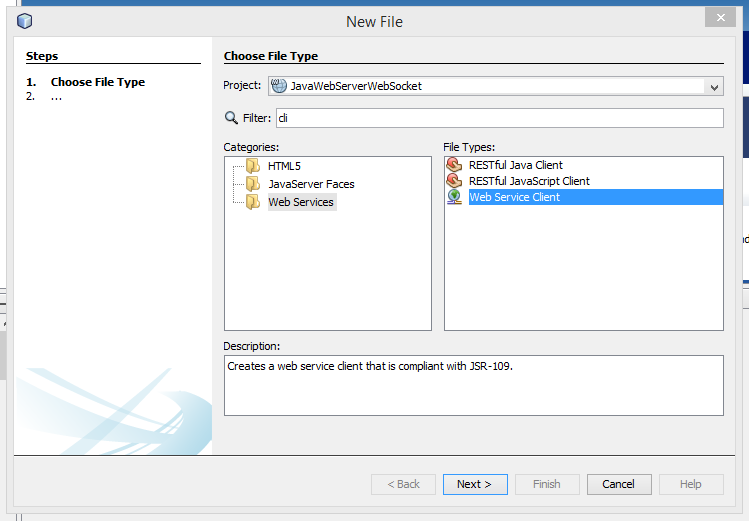
\includegraphics[width=0.9\textwidth]{Figures/client1.png}
  \caption[Step 1 to generate client code from WSDL file.]{Step 1 to generate client code from WSDL file..}
  \label{fig:wsdlstep1}
\end{figure}
\begin{figure}[!htb]
  \centering
  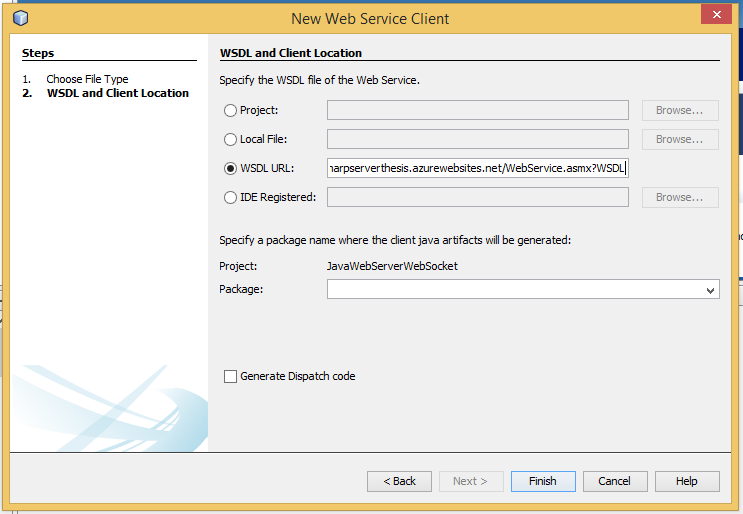
\includegraphics[width=0.9\textwidth]{Figures/client2.png}
  \caption[Step 2 to generate client code from WSDL file.]{Step 2 to generate client code from WSDL file..}
  \label{fig:wsdlstep2}
\end{figure}

As seen in Listing ~\ref{lst:wsdldocument} for very basic example there is a big WSDL document in case using SOA architecture.

As seen with examples, a typical and pragmatic solution is to resort to Web Services and XML data, sharing schemas and namespaces, or to RESTful APIs, which are simpler to use and require that schemas (media types) be standardized or pre-agreed. In these technologies, both customer and provider are forced to implement full interoperability (for example, sharing a XML schema), even if only a fraction of the possible interactions is used. This leads to a greater coupling than needed. In Chapter \ref{chapter:architecture}, the proposed solution  reduce coupling with using partial interoperability and creating the maximum decoupling possible while ensuring the minimum interoperability requirements.
